\chapter{Adaptive Optik\label{chapter:thema}}
\lhead{Adaptive Optik}
\begin{refsection}
\chapterauthor{Matthias Schneider}

\section{Einleitung}
In diesem Kapitel wird das Thema Adaptive Optik behandelt, dazu werde ich zuerst eine kurze Übersicht über das Thema geben und anschliessend einige Aspekte genauer erklären und dazu auch mathematische Herleitungen machen. 

\section{Adaptive Optik und ihre Anwendungen}
Adaptive Optik (AO) ist eine Technik mit der optische Systeme verbessert werden können. Dabei können aber nur Fehler korrigiert werden, welche im Medium zwischen der Quelle des Lichtes und dem Sensor entstehen, hauptsächlich geht es also darum, Fehler die durch die Atmosphärenunruhe entstehen zu kompensieren. Die erdgebundene Astronomie ist heute auf diese Technologie angewiesen, denn Beobachtungen im optischen und infraroten Bereich sind nur möglich, wenn die negativen Effekte der Atmosphäre korrigiert werden können. Ein schönen Beispiel dazu ist die Aufnahme vom Jupiter mit dem Very Large Telescope (VLT) der European Southern Observatory (ESO).

\begin{figure}
  \centering
  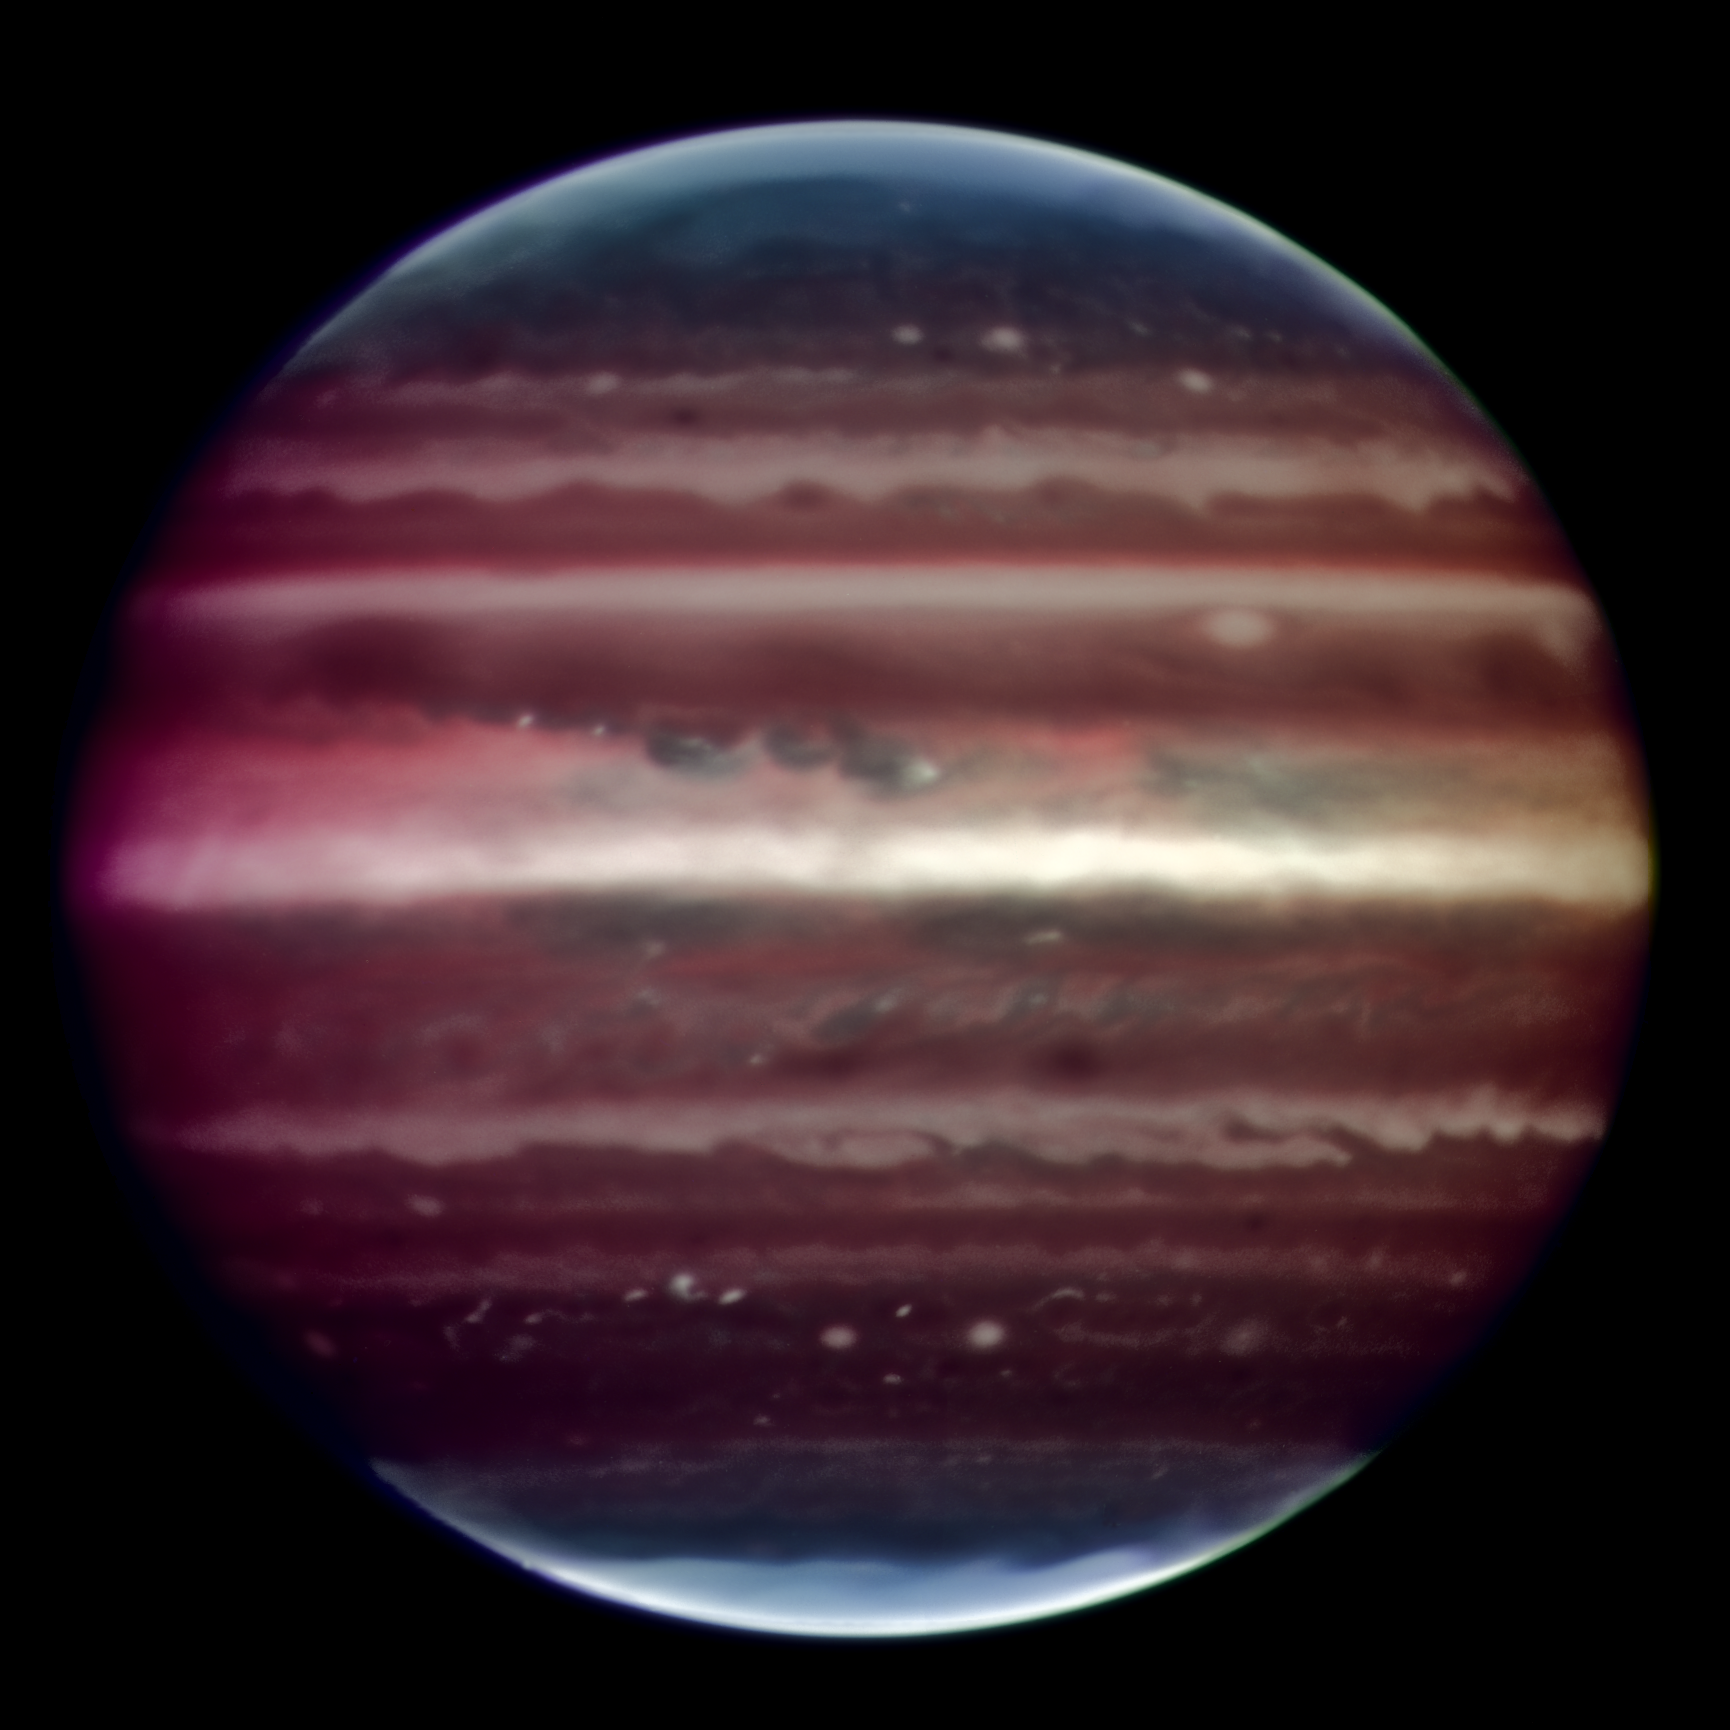
\includegraphics[width=0.5\textwidth]{adaptiv/images/Jupiter_adaptiv}
  \caption{Jupiter mit adaptiver Optik von der Erde aus mit VLT aufgenommen
    \cite{eso:jupiter}}
  \label{fig:jupiter}
\end{figure}

Adaptive Optik wird heute aber auch bei anderen Anwendungen eingesetzt, um die Präzision von Optischen Apparaturen zu erhöhen, so gibt es heute Mikroskope mit AO. Ein weiterer Einsatzbereich dieser Technologie ist der Fokusiserspiegel von Laserschneidanlagen, womit eine deutliche Steigerung der Präzision beim schneiden erreicht wird.\newline
Die Technologie ist aus drei Hauptkomponenten aufgebaut, es braucht einen Sensor, der die Störung der Wellenfront messen kann, einen Computer der die benötigte Korrektur berechnet und einen beweglichen Spiegel, mit welchem die Wellenfront korrigiert werden kann, damit dann auf den Messinstrument ein möglichst scharfes Bild entsteht.\newline
Als Sensor wird für gewöhnlich eine Hartmannplatte verwendet, welche aus einem Mikrolinsenarray besteht und pro Linse einen CMOS oder CCD-Sensor, mit welchem die Verkippung der Wellenfront im Bereich einer einzelnen Linse bestimmt werden kann. 

\begin{figure}
  \centering
  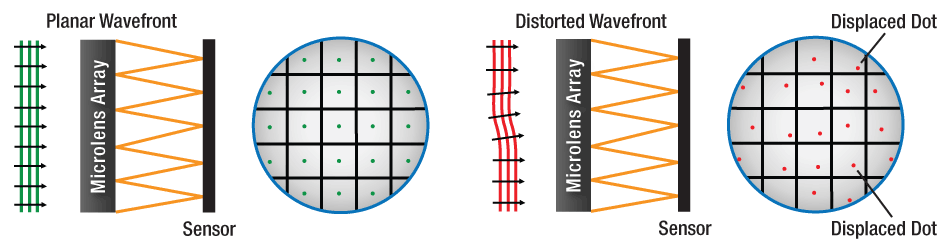
\includegraphics[width=0.9\textwidth]{adaptiv/images/hartmannplatte}
  \caption{Hartmannplatte mit ebener und verformter Wellenfront
    \cite{thor:hartmannplatte}}
  \label{fig:hartmannplatte}
\end{figure}

Ein weiteres wichtiges Element bei der adaptiven Optik ist das Erzeugen einer Referenzquelle, welche ein Signal erzeugt, dass bekannt ist und so der Einfluss der Atmosphäre gemessen werden kann. In der Astronomie wird dazu mit Laser ein künstlicher Stern erzeugt, dieser sogenannte Leitstern wird in einer Höhe von etwa 90$km$ erzeugt, also am oberen Ende der Mesosphäre. Dazu wird oft ein Natrium-Laser verwendet, der eine Wellenlänge von 589$nm$ hat. Dieses Licht wird dann von den Natriumatomen in der Höhe von 90$km$ zurückgeworfen. Dabei wird die Annahme gemacht, dass dabei ein Stern entsteht, dessen Licht sich Kugelförmig ausbreitet. 

\begin{figure}
  \centering
  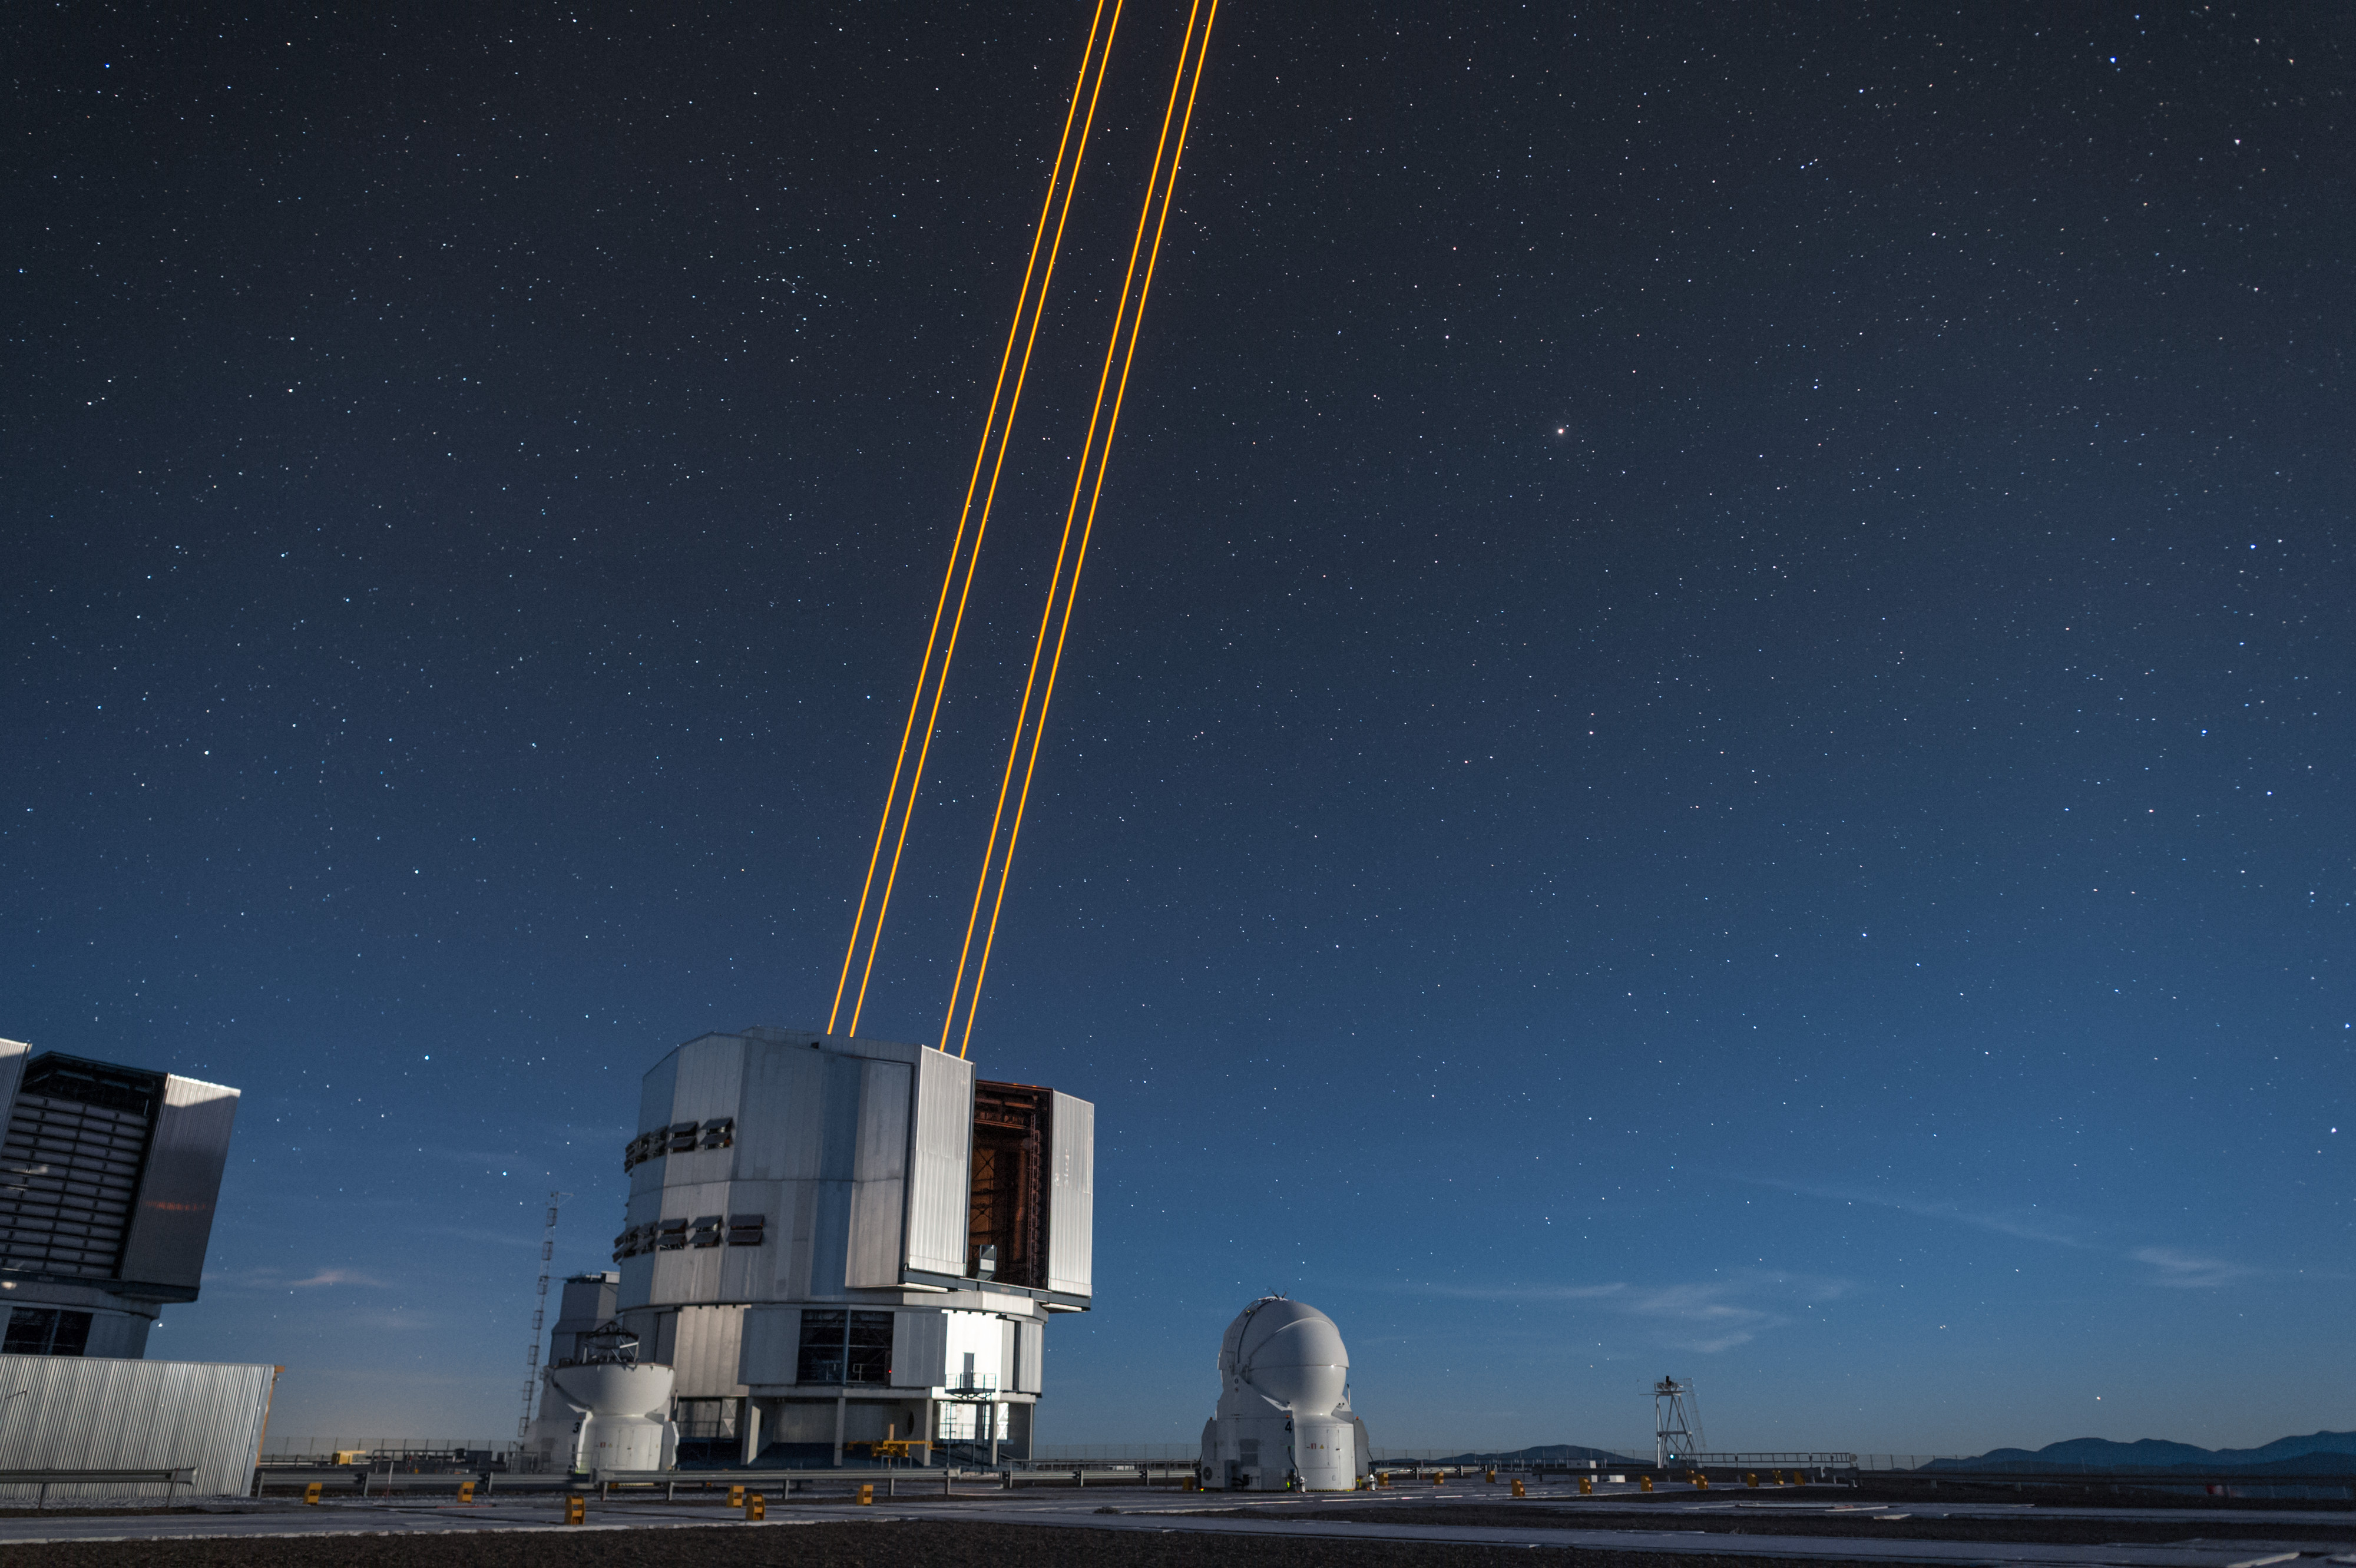
\includegraphics[width=0.5\textwidth]{adaptiv/images/Leitstern}
  \caption{Erzeugung eines Leitsterns (VLT der ESO Paranal Observatorium)
    \cite{eso:leitstern}}
  \label{fig:hartmannplatte}
\end{figure}

\section{Kürzester Weg}
Wenn wir zwei Punkte im Raum betrachten und den kürzesten Weg zwischen ihnen suchen, so würden wir intuitiv die Punkte mit einer Geraden verbunden und diesen Weg als den kürzesten definieren. Wenn nun aber das Licht den kürzesten Weg zwischen zwei Punkten geht, wird nicht wie beim klassischen Weg die Strecke minimiert, sondern die Laufzeit die das Licht benötigt. Das führt dazu, dass wenn zwischen den zwei Punkten eine Phasengrenze liegt, der Weg nicht mehr die direkte Verbindung ist sondern eine Streckt die in etwa so aussieht Dieses Verhalten wird von Fermat's Prinzip beschrieben.

\begin{figure}
  \centering
  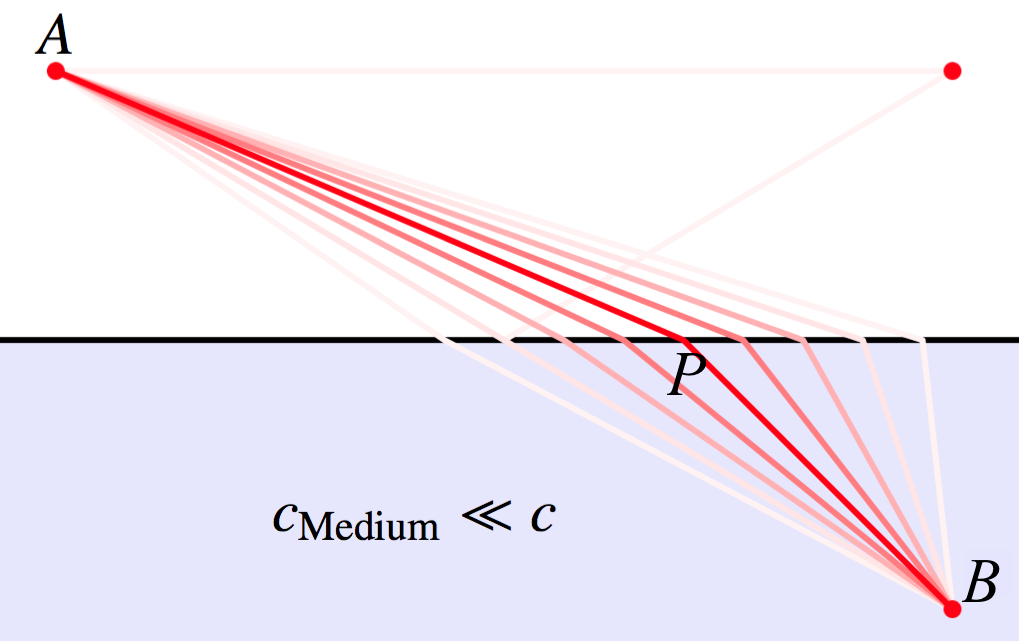
\includegraphics[width=0.5\textwidth]{adaptiv/images/Weg}
  \caption{Kürzester Weg zwischen zwei Punkten}
  \label{fig:weg}
\end{figure}

Welchen weg nimmt nun aber das Licht, wenn es wie auf der Abbildung \ref{fig:weg} von A nach B muss und dazwischen ein Übergang des Mediums stattfindet, somit das Licht nicht den intuitiv direkten Weg gehen kann. Nach dem Prinzip von Fermat muss also die Zeit auf $\overline{AP}$ und $\overline{PB}$ minimal sein. Es muss also die Gleichung \eqref{bedmin} erfüllt sein, damit die Laufzeit minimal wird

\begin{equation}\label{bedmin}
\dfrac{\partial t}{\partial p_{x}}=0
\end{equation}
Um $t$ zu bestimmen werden nun die Strecken $\overline{AP}$ und $\overline{PB}$ benötigt. Dabei haben die Punkte die folgenden Koordinaten $A = (0,a)$, $P=(p_{x},p_{y})$ und $B=(b,0)$. Die Gleichung \eqref{tbest} erklärt, wie aus Abblidung \ref{fig:weg} die jeweiligen Strecken bestimmt werden können. In einem weiteren Schritt wird die Gleichung \eqref{tbest} partiell nach $p_{x}$ abgeleitet und die Ableitung gleich Null gesetzt.

\begin{equation}\label{tbest}
t=\dfrac{s}{s}=\dfrac{\overline{AP}}{v_{1}}+\dfrac{\overline{PB}}{v_{2}}= 
\dfrac{\sqrt{(a-p_{y})^{2}+p_{x}^{2}}}{v_{1}}+ 
\dfrac{\sqrt{(b-p_{x})^{2}+p_{y}^{2}}}{v_{2}}
\end{equation}

\begin{equation}\label{partdiff}
\dfrac{\partial t}{\partial p_{x}}=0 \Rightarrow 
\dfrac{1}{v_{1}}\cdot \dfrac{1}{2 \sqrt{(a-p_{y})^{2}+p_{x}^{2}}}\cdot 2p_{x} +
\dfrac{1}{v_{2}}\cdot \dfrac{-1}{2 \sqrt{(b-p_{x})^{2}+p_{y}^{2}}}\cdot 2(b-p_{x})= 0
\end{equation}

Die Geschwindigkeit $ v_{1} = \frac{c}{n_{1}} $ und $ v_{2} = \frac{c}{n_{2}}$ ist dabei die Lichtgeschwindigkeit im jeweiligen Medium. Wird nun in die Gleichung \eqref{partdiff} $ v_{1}$ und $ v_{2}$ eingesetzt und anschliessend mit $c$ multipliziert, erhält man die Gleichung \eqref{glp1} aus welchen dann der Punkt $P$ bestimmt werden kann und somit der Strahlengang von $A$ nach $B$ via $P$ bestimmt ist. Dieser Weg ist nun minimal bezüglich der Laufzeit. Zur besseren Verständlichkeit noch eine kleiner Vergleich:\newline
Es ist nun kein Photon das den Weg zurücklegen muss, sondern ein ausgesprochen intelligenter Hund der bei $A$ startet und bei $B$ einen Ball im Wasser holen muss, die schwarz horizontale Linie auf der Abbildung \ref{fig:weg} ist dabei das Ufer. Wenn nun der Hund den zuvor beschrieben Weg wählt, ist er am schnellsten beim Ball der Grund ist, er rennt an Land schneller als er schwimmen kann. Der Punkt $P$ ist also der optimale Punkt für den Hund um uns Wasser zu springen.

\subsection{Warum der kürzeste Weg}
Auf dem Weg von der Lichtquelle, in der Astronomie sind das oft Sterne, Sternhaufen, Galaxien oder sogar ganze Cluster von Galaxien, trifft das Licht immer wieder auf Störeinflüsse. Störungen die auf dem Weg durch dass All entstehen werden im nächsten Kapitel besprochen, in diesem Abschnitt geht es ja um Störungen die in der Atmosphäre entstehen. Wenn mit einem Teleskop Sterne beobachtet werden kann man immer von sehr gutem Wetter ausgehen und trotzdem ist die Atmosphäre vielschichtig aufgebaut. Das Licht sucht sich nun den schnellsten Weg durch die verschiedenen Schichten, dabei ist bei jedem Übergang zwischen zwei Schichten auch zu "Richtungsänderung" des Lichtes wie auf Abbildung \ref{fig:weg}.

\section{Wellenfront}



\printbibliography[heading=subbibliography]
\end{refsection}

